\documentclass[conference]{IEEEtran}

\usepackage{amsmath,amssymb,amsfonts}
\usepackage{algorithm}
\usepackage{algpseudocode}
\usepackage{graphicx}
\usepackage{textcomp}
\usepackage{mathtools}
\usepackage{commath}
\usepackage[style=numeric, backend=bibtex, language=english, maxbibnames=99]{biblatex}

% tikz
\usepackage{tikz}
\usetikzlibrary{shapes.geometric, arrows}
% tikz styles
\tikzstyle{user} = [circle, thick, draw, minimum size=2.5cm]
\tikzstyle{item} = [rectangle, thick, draw, minimum width=3cm, minimum height=1.5cm]
\tikzstyle{arrow} = [->, draw, thick]
\tikzstyle{bi-arrow} = [<->, draw, thick]
\tikzstyle{line} = [-, draw, thick]

\def\BibTeX{{\rm B\kern-.05em{\sc i\kern-.025em b}\kern-.08em
    T\kern-.1667em\lower.7ex\hbox{E}\kern-.125emX}}

\emergencystretch=8em

\bibliography{literature}

\begin{document}

\title{Community Embeddings for Friend Suggestions}

\author{
    \IEEEauthorblockN{Anton I. N. Begehr}
    \IEEEauthorblockA{
        \textit{Graduate School of Business}\\
        \textit{National Research University Higher School of Economics}\\
        Moscow, Russia\\
        a.begehr@fu-berlin.de\\
    }
    \and
    \IEEEauthorblockN{Prof. Dr. Petr Panfilov}
    \IEEEauthorblockA{
        \textit{Graduate School of Business}\\
        \textit{National Research University Higher School of Economics}\\
        Moscow, Russia\\
        ppanfilov@hse.ru\\
    }
}

\maketitle

\begin{abstract}
    Graphs, such as social networks, emerge naturally from various real-world situations. Recently, graph embedding methods have gained traction in data science research.
    Recommender systems are used in a wide range of business applications and are essential for online, e-business models to survive and strive in the contemporary market. Using graph embeddings for recommendation tasks, have the possibility of improving upon recommender systems, because of data compression, their feature vector format, and sub-quadratic time complexity.
    Graph and community embeddings generated with ComE BGMM+VI are used to build a recommender system for friend suggestions. ComE BGMM+VI is an alteration of the community embeddings algorithm ComE. ComE BGMM+VI applies a Bayesian Gaussian mixture model and variational inference for community embedding and detection.
    Recommendations are evaluated by the top-N hit-rate over users with at least 50 friends. A friend suggestions recommender system with a top-10 leave-one-out hit-rate of 43.6\% and run-time optimized 32.9\% is presented.
\end{abstract}

\begin{IEEEkeywords}
    graph, embedding, community embedding, ComE, recommendations, friend suggestions
\end{IEEEkeywords}


\section{Introduction}

Graphs, such as social networks, knowledge graphs, content-rating graphs, and communication networks, emerge naturally from various real-world situations. Analyzing these graphs leads to findings and understanding of the underlying structures, coherences, and dependencies. Recently, methods for embedding graph's nodes into lower-dimensional Euclidean spaces, called graph embeddings, have gained traction in multiple areas of data science research \cite{Goyal_2018}.

Due to the rapid growth of the internet and data accumulation, recommender systems are essential for e-business and online business models to survive and strive in the contemporary market \cite{Polatidis2013RecommenderST}. Modern recommender systems need to take into account the huge amounts of user data generated at all times in big data systems around the world and improve recommendations instead of failing under the thrust of big data overload.

Utilizing graph embeddings for recommendation tasks, has recently gained research traction \cite{Palumbo2018AnEC, Palumbo2018KnowledgeGE, GradGyenge2017GraphEB, Sathish2019GraphEB}. The advantages of graph embeddings include data compression and the Euclidean feature vector format \cite{Godec2018}. Given these advantages and provided competitive results, graph embeddings have the possibility of greatly improving upon graph-based use-cases like recommender systems.

Community Embeddings, in addition to embedding a graph's nodes through first- and second-order proximity, also preserve higher-order proximity by embedding clusters present in the graph data. The graph and community embedding algorithm ComE aims to preserve first-, second- and higher-order proximity by embedding a graph's nodes and communities \cite{ComE}.

This work specifically examines community embeddings for friend suggestion recommender systems and evaluates recommendations on social network graph data for the use-case of friend suggestions. Graph and community embeddings generated with ComE BGMM+VI are used to develop a friend suggestions recommender system based on the shortest distances between nodes in the embedding. Recommendations are evaluated by the top-$N$ recommendations hit-rate of test edges. A friend suggestions recommender system with a top-10 leave-one-out hit-rate of 43.6\% and run-time optimized 32.9\% is presented.


\section{Friend Suggestions}

Recommender Systems are eagerly researched in academia and widely deployed in real-world business applications. Most contemporary technology companies heavily rely on recommender systems to drive usage of their services and consumption of their content. Users, in turn, rely on recommender systems to find what they want and need and save searching time. State-of-the-art recommender systems provide a competitive advantage desperately needed by online services. Companies heavily relying on recommender systems include YouTube, Amazon, Netflix, and many more \cite{Rocca19}.

Recommender systems are built on top of user-item interaction. Friend suggestions are a simpler type of recommender system. For friend suggestions, no distinction is made between users and items. The entity user is both the subject and object of recommendation. This results in a simple data model, which can be used for structural friend suggestions, as shown in Fig. \ref{fig:data_model}:

\begin{figure}[H]
    \centering
    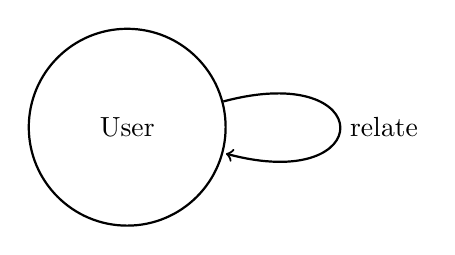
\begin{tikzpicture}[node distance=6cm]
        \node (user) [user] {User};
        \path [arrow] (user) edge[loop right] node[right]{relate} (user);
    \end{tikzpicture}
    \caption{Minimal data model supporting friend suggestions.}
    \label{fig:data_model}
\end{figure}

The two main methods used for recommender systems are collaborative filtering and content-based filtering. Collaborative filtering is based on the assumption that users like items similar to other items they like and items that are liked by other users with similar tastes \cite{Grover17, Su2009ASO}. Content-based filtering considers user and item attributes, instead of solely interactions \cite{Rocca19, Lops2011SurveyCB}.

In this paper, a method of generating friend suggestions based solely on graph data structure, and not on the node or edge attributes, is presented. The graph of users and friendships is embedded to a lower-dimensional space with the community embedding algorithm ComE BGMM+VI \cite{ComE, ComE+, ComE_BGMM_GH}. The approach can be considered a variant of collaborative filtering with the euclidean distance of user embeddings and user community membership as measures for user similarity. The proposed advantage of using such an approach is that community embeddings optimize first-, second-, and higher-order proximity between users in the node embedding.

\subsection{Evaluation}

To determine the effectivity of friend suggestions, the generated friend suggestions must be properly validated. In this paper, the top-$N$ approach to evaluating recommender systems with hit-rate as the evaluation metric is chosen.

A user's top-$N$ recommendations is a list of $N$ items to be recommended to a specific user. To evaluate recommender systems with the top-$N$ and hit-rate approach, initially, the dataset is split into train and test data. For each testing user, one relation is left out, according to the leave-one-out method and the model is trained on the remaining training dataset. Once the model is trained, a list of top-$N$ recommendations is generated for each testing user. If the item corresponding to the user is in the user's top-$N$ list, a hit is counted, otherwise, a miss is counted. The hit-rate is defined as the total number of hits divided by the number of testing users.

Utilizing the top-$N$ approach with hit-rate to evaluate recommender systems is advantageous to evaluating recommender systems by a link prediction approach since the top-$N$ approach is more realistic in comparison to actual recommender system use-cases. When you open Netflix, Amazon, YouTube, or Facebook friend suggestions, one or multiple top-$N$ recommendation lists are generated and displayed. If you click on an item and buy, watch, or befriend, that is considered a hit, otherwise, a miss.

The hit-rate metric on top-$N$ recommendations provides a realistic option of evaluating recommender systems \cite{Cremonesi2010PerformanceOR, Palumbo2017entity2rec, Zhao2019ATS}.


\section{Algorithm}

The proposed algorithm for generating friend suggestions using community embeddings is detailed and evaluated on time complexity. The initially quadratic runtime of generating friend suggestions for all users is then reduced by a factor of $K$ by utilizing a node's community membership. The two resulting algorithms are presented.

Algorithm \ref{alg:friend_sug} describes in pseudocode how recommendations are computed from node embeddings generated by ComE BGMM+VI. The terms friend suggestions and social recommendations are used interchangeably.

\begin{algorithm}
    \caption{Top-$N$ Social Recommendations based on Node Embeddings}
    \label{alg:friend_sug}
    \begin{algorithmic}[1]
        \Require{graph $G = (V, E)$, maximum number of communities K, number of walks $\gamma$, walk length $\ell$, window size $\zeta$, representation size $D$, negative context size $m$, parameters ($\alpha$, $\beta$), number of recommendations $N$.}
        \Ensure{Top-$N$ recommendations for all nodes $R$.}
        % run ComE BGMM+VI
        \State $\Phi, \Phi', \Pi, (\Psi,\Sigma) \leftarrow ComE(G, K, \gamma, \ell, \zeta, D, m, \alpha, \beta)$
        % find friends
        \For{$(v, v') \in E$}
        \State $F_v \leftarrow F_v \cup \{v'\}$
        \State $F_{v'} \leftarrow F_{v'} \cup \{v\}$
        \EndFor
        % for each node
        \For{$v \in V$}
        % generate ascending recommendation list for each node
        \State $R_v \leftarrow SortedDict(size=N)$
        \For{$v' \in V \land v' \notin F_v \land v' \neq v$}
        \State $d \leftarrow \|\phi_v - \phi_{v'}\|$
        \State $R_v[d] \leftarrow v'$
        \EndFor
        % get Top-N recommendations for each node
        \State $R_v  \leftarrow R_v.values()$
        \EndFor
    \end{algorithmic}
\end{algorithm}

The function $ComE(G, K, \gamma, \ell, \zeta, D, m, \alpha, \beta)$ is the ComE BGMM+VI community embedding algorithm. It returns the node embedding $\Phi$, context embedding $\Phi'$, community assignment $\Pi$, and community embedding $(\Psi,\Sigma)$. ComE BGMM+VI is based on the ComE algorithm presented by \citeauthor{ComE} in their paper \citetitle{ComE} as algorithm 1 on page 381 of the publication's in-proceeding \cite{ComE}. ComE BGMM+VI takes a Bayesian approach to community embedding by utilizing  a Bayesian Gaussian mixture model (BGMM) and variational inference (VI) for community embedding and detection instead of a non-Bayesian Gaussian mixture model (GMM) with expectation maximization (EM) \cite{ComE_BGMM_GH}. %TODO citation to the ComE BGMM paper.

The runtime of ComE BGMM+VI is equivalent to the runtime of ComE in its big-$O$ notation. ComE's time complexity is $O(\abs{V}\gamma\ell + \abs{V} + T_1 (T_2\abs{V}K + K + \abs{E} + \abs{V}\gamma\ell + \abs{V}K))$, which is linear in time complexity to the graph size: $O(\abs{V} + \abs{E})$ (line 1) \cite{ComE}. All friends of each user are determined in $O(E)$ (lines 2-5). A sorted dictionary of the top-$N$ friend suggestions for each user sorted ascending by distances between the node embeddings is computed in $O(\abs{V}^2N))$ (lines 6-13). Top-$N$ friend suggestions are generated for each user: $O(\abs{V})$. For each user, all users not befriended currently are considered ($O(\abs{V})$) and inserted into a sorted dictionary of length $N$ ($O(N)$).

This brings the total time complexity of Algorithm \ref{alg:friend_sug} to $O(\abs{V}\gamma\ell + \abs{V} + T_1 (T_2\abs{V}K + K + \abs{E} + \abs{V}\gamma\ell + \abs{V}K) + \abs{E} + \abs{V}^2N)$. We consider $\gamma$, $\ell$, $T_1$, $T_2$, and $N$ as constant, therefore the time complexity depends on the graph's size $(\abs{V}, \abs{E})$ and the number of communities $K$: $O(K + \abs{V}K + \abs{E} + \abs{V}^2)$.

Algorithm \ref{alg:friend_sug_com} describes in pseudocode how recommendations are computed from ComE BGMM+VI node and community embeddings and community assignments. The advantage of also considers community membership, is that an improvement in time complexity can be obtained, by considering only users in the same community for friend suggestions.

\begin{algorithm}
    \caption{Top-$N$ Social Recommendations based on Node and Community Embeddings}
    \label{alg:friend_sug_com}
    \begin{algorithmic}[1]
        \Require{graph $G = (V, E)$, maximum number of communities K, number of walks $\gamma$, walk length $\ell$, window size $\zeta$, representation size $D$, negative context size $m$, parameters ($\alpha$, $\beta$), number of recommendations $N$.}
        \Ensure{Top-$N$ recommendations for all nodes $R$.}
        % run ComE BGMM+VI
        \State $\Phi, \Phi', \Pi, (\Psi,\Sigma) \leftarrow ComE(G, K, \gamma, \ell, \zeta, D, m, \alpha, \beta)$
        %  generate a set of nodes for each community
        \For{$v \in V$}
        \State $k \leftarrow \pi_v$
        \State $C_k \leftarrow C_k \cup \{v\}$
        \EndFor
        % find friends
        \For{$(v, v') \in E$}
        \State $F_v \leftarrow F_v \cup \{v'\}$
        \State $F_{v'} \leftarrow F_{v'} \cup \{v\}$
        \EndFor
        % for each node
        \For{$v \in V$}
        % generate ascending recommendation list for each node
        \State $R_v \leftarrow SortedDict(size=N)$
        \For{$v' \in C_k \land v' \notin F_v \land v' \neq v$}
        \State $d \leftarrow \|\phi_v - \phi_{v'}\|$
        \State $R_v[d] \leftarrow v'$
        \EndFor
        % get Top-N recommendations for each node
        \State $R_v  \leftarrow R_v.values()$
        \EndFor
    \end{algorithmic}
\end{algorithm}

Line 1, lines 6-9, and lines 10-17, except for line 12, are the same in Algorithm \ref{alg:friend_sug_com} as in Algorithm \ref{alg:friend_sug}. All users are filtered into sets $C_k$, one for each community $k$ in $O(\abs{V})$ (lines 2-5). Instead of considering the set of all non-friends users of size $\abs{V}$, only users in the same community $C_k$ of size $\frac{\abs{V}}{K}$ are considered (line 12) in $O(\frac{\abs{V}^2N}{K})$.

This brings the total time complexity of Algorithm \ref{alg:friend_sug_com} to $O(\abs{V}\gamma\ell + \abs{V} + T_1 (T_2\abs{V}K + K + \abs{E} + \abs{V}\gamma\ell + \abs{V}K) + \abs{V} + \abs{E} + \frac{\abs{V}^2N}{K})$. Again, we consider $\gamma$, $\ell$, $T_1$, $T_2$, and $N$ as constant, therefore the time complexity depends on the graph's size $(\abs{V}, \abs{E})$ and the number of communities $K$: $O(K + \abs{V}K + \abs{E} + \frac{\abs{V}^2}{K})$.

The hyper-parameter number of communities $K$ can reduce the quadratic summand $\abs{V}^2N$ by only considering users of the same community for friend suggestions. The reduction in time complexity through Algorithm \ref{alg:friend_sug_com} is only scalable when considering $K$ to be scale with the input graph's size. This assumption can be made when considering communities as groups of friends: with ten times more users, these users form ten times more communities.


\section{Visual Example}








%%% Bibliography
\printbibliography

\end{document}
